\documentclass{beamer}

\mode<presentation>
  {\usetheme{MooijTalk}}
\definecolor{beamer@blendedblue}{rgb}{0.0,0.47,0.44}
%\definecolor{beamer@blendedblue}{rgb}{0.75,0.19,0.10}
\usepackage{appendixnumberbeamer}
\setbeamercovered{invisible}
%\setbeamercolor*{example text}{fg=blue!50!black}
\setbeamercolor*{example text}{fg=beamer@blendedblue}

\usepackage{bbding}
\usepackage{tikz}
\usetikzlibrary{arrows}
\usetikzlibrary{patterns}
\usetikzlibrary{backgrounds}
\usetikzlibrary{decorations.pathmorphing}
\usetikzlibrary{positioning}

\newdimen\arrowsize
\pgfarrowsdeclare{arcsq}{arcsq}
{
  \arrowsize=0.2pt
  \advance\arrowsize by .5\pgflinewidth
  \pgfarrowsleftextend{-4\arrowsize-.5\pgflinewidth}
  \pgfarrowsrightextend{.5\pgflinewidth}
}
{
  \arrowsize=1.5pt
  \advance\arrowsize by .5\pgflinewidth
  \pgfsetdash{}{0pt} % do not dash
  \pgfsetroundjoin   % fix join
  \pgfsetroundcap    % fix cap
  \pgfpathmoveto{\pgfpoint{0\arrowsize}{0\arrowsize}}
  \pgfpatharc{-90}{-160}{4\arrowsize}
  \pgfusepathqstroke
  \pgfpathmoveto{\pgfpointorigin}
  \pgfpatharc{90}{160}{4\arrowsize}
  \pgfusepathqstroke
}

\usepackage{bm}
\usepackage{graphicx}
\usepackage{url}
\usepackage{algorithm}
\usepackage{algorithmic}
\usepackage{latexsym}
\usepackage{comment}
\usepackage{amsfonts}
\usepackage{amsmath}
\usepackage{mymacros}
\usepackage[english]{babel}

\graphicspath{{fig/}}

\definecolor{mpglogogreen}{RGB}{0,124,121}
\definecolor{mpgdarkgreen}{RGB}{124,166,166}
\definecolor{mpgmidgreen}{RGB}{201,219,216}
\definecolor{mpglightgreen}{RGB}{230,242,242}
\definecolor{mpgdarkgray}{RGB}{102,102,102}
\definecolor{mpgalert}{RGB}{204,51,40} % red
\definecolor{mpi}{rgb}{0.0,0.47,0.44}
\definecolor{ru}{rgb}{0.75,0.19,0.10}

\title[Causality]{Causality: Overview}
\author[Joris Mooij]{\\[5mm]\large Joris Mooij \& Patrick Forr\'e\\
\url{j.m.mooij@uva.nl}, \url{p.d.forre@uva.nl}}
\institute[UvA]{
\begin{tikzpicture}
%  \node at (0,0) {\includegraphics[height=15mm]{amlab}};
  \node at (6,0) {\includegraphics[height=7mm]{uva_logo_en}};
%  \node[text width=4cm,text centered] at (0,1) {\small Institute for Computing\\ and Information Sciences};
%  \node[text width=4cm,text centered] at (7,1) {\small Informatics Institute};
\end{tikzpicture}}
\date[2021-02-02]{\normalsize February 2, 2021}

\DeclareMathOperator{\intervene}{do}
\newcommand\ddadbdc[3]{\frac{\partial^2 #1}{\partial #2 \partial #3}}
\newcommand\rowvector[1]{\left( \begin{array}{c} #1 \end{array} \right)}
\newcommand\de[1]{\mathrm{de}({#1})}
\newcommand\at{\Bigg|}
\newcommand\M[1]{\mathbf{\mathsf{#1}}}
\newcommand\myexample[1]{{\color{blue}#1}}
\def\imagetop#1{\vtop{\null\hbox{#1}}}

\newcommand{\ot}{\leftarrow}
\newcommand{\oto}{\leftrightarrow}
\newcommand{\ots}{\leftarrow\mkern-13mu\ast\,}
\newcommand{\sto}{\,\ast\mkern-13mu\to}
\newcommand{\stt}{\,\ast\mkern-13mu\relbar\!\!\!\relbar}
\newcommand{\tts}{\relbar\!\!\!\relbar\mkern-13mu\ast\,}

\tikzstyle{var}=[circle,draw=black,fill=white,thick,minimum size=20pt,inner sep=0pt]
\tikzstyle{varc}=[draw=black,fill=white,thick,minimum size=20pt,inner sep=0pt]
\tikzstyle{varh}=[circle,draw=gray,fill=gray!10,thick,minimum size=20pt,inner sep=0pt,dotted]
\tikzstyle{arr}=[->,>=stealth',draw=black,thick]
%\tikzstyle{arr}=[->,>=stealth',draw=black,fill=black,line width=1pt]
%\tikzstyle{arrh}=[->,>=stealth',draw=gray,thin]
\tikzstyle{arrh}=[->,>=stealth',draw=gray,fill=gray,thick,dotted]
\tikzstyle{biarr}=[<->,>=stealth',draw=black,fill=black,thick]
\tikzstyle{biarrh}=[<->,>=stealth',draw=gray,fill=gray,thick,dotted]
\tikzstyle{fac}=[rectangle,draw=black!50,fill=black!20,thick,minimum size=10pt] %or 15pt
\tikzstyle{vari}=[circle,draw=white,fill=red,thick,minimum size=20pt,inner sep=0pt]

\begin{document}

\maketitle

\frame{\frametitle{Many questions in science are \emph{causal}}
  \begin{tikzpicture}
    \node at (-0.3,2.5) {\textbf{Climatology}:};
    \node at (-0.3,0) {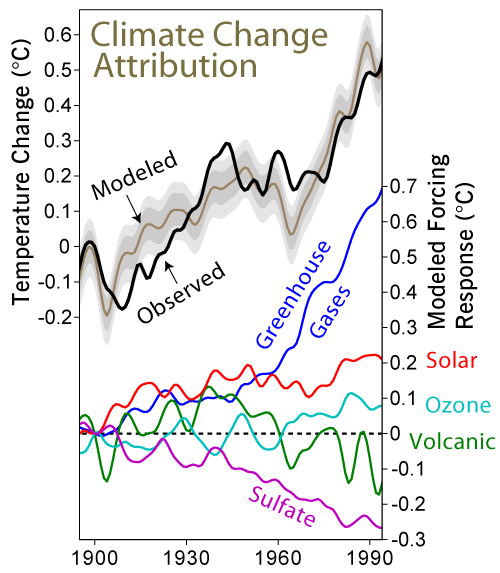
\includegraphics[height=4cm]{Climate_Change_Attribution.png}};
    \node at (6,2.5) {\textbf{Economy}:};
    \node at (6,0)  {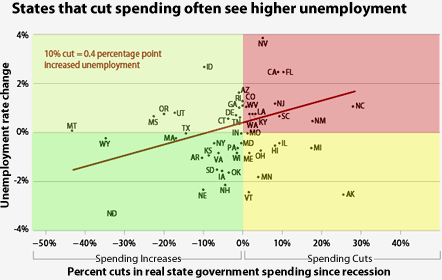
\includegraphics[height=4cm]{state-spending-cuts-unemployment}};
    \node at (6,-2.5) {\textbf{Neuroscience}:};
    \begin{scope}[transform canvas={scale=0.6},xshift=6.5cm,yshift=-7cm]
      \node at (0.3,0) {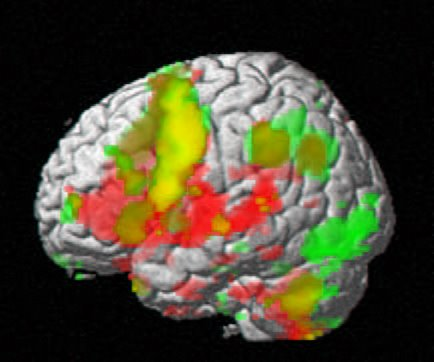
\includegraphics[height=3.8cm]{fmri.jpg}};
      \node at (6.7,0) {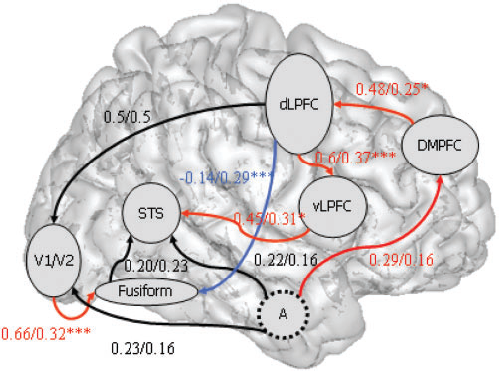
\includegraphics[height=4cm]{connectivity.png}};
      \draw[->, >=latex, line width=6pt] (2.7,0) -- (4.2,0);
    \end{scope}
    \node at (-0.3,-2.5) {\textbf{Medicine}:};
    \node at (-0.3,-4.2) {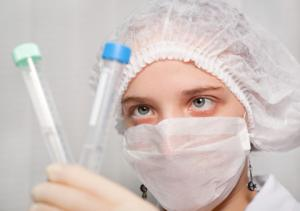
\includegraphics[height=2.2cm]{clinical.jpg}};
  \end{tikzpicture}
%  \nocite{MooijJanzingSchoelkopf_UAI_13}
}

\frame{\frametitle{Lecture contents}
  Causality is clearly an important notion in daily life and in science.  But,
  \begin{itemize}
    \item How can we formalize the notion of causality with \textbf{causal models}?
    \item How to \textbf{reason} about causality?
    \item How can we \textbf{discover} causal relations from data?
    \item How to obtain causal \textbf{predictions}?
    \item How do they differ from ordinary predictions in stats/ML?
  \end{itemize}

  \bigskip
  That is what you will learn in these lectures!
}

\frame{\frametitle{Probabilistic Inference vs.\ Causal Inference}
  \textbf{Probabilistic Inference (traditional statistics / machine learning)}
  \begin{itemize}
%  \item About \emph{associations} %(\myexample{correlation between smoking and lung cancer}) 
  \item Models the \alert{distribution} of the data
  \item Focuses on predicting from \alert{observations} %(\myexample{if we \alert{observe} that somebody smokes, what is the probability that he/she gets lung cancer?}) 
  \item Useful e.g.\ in medical diagnosis: \emph{given the symptoms of the patient, what is the most likely disease?}
  \end{itemize}

%  \pause
  \medskip
  \textbf{Causal Inference}\\
  \begin{itemize}
%  \item About \emph{causation} %(\myexample{smoking causes lung cancer})
  \item Models the \alert{mechanism} that generates the data
  \item Also allows to predict results of \alert{interventions} %(\myexample{if we \alert{force} somebody to smoke, what is the probability that he/she will get lung cancer?}) 
  \item Useful e.g.\ in medical treatment: \emph{if we treat the patient with a drug, will it cure the disease?}
  \end{itemize}

%  \pause
  \begin{block}{}
  Causal reasoning is essential to answer questions of the type: \emph{given the circumstances, what action should we take to achieve a certain goal?}
  \end{block}

}

\begin{frame}{Causality: an Active Research Area}\centering
  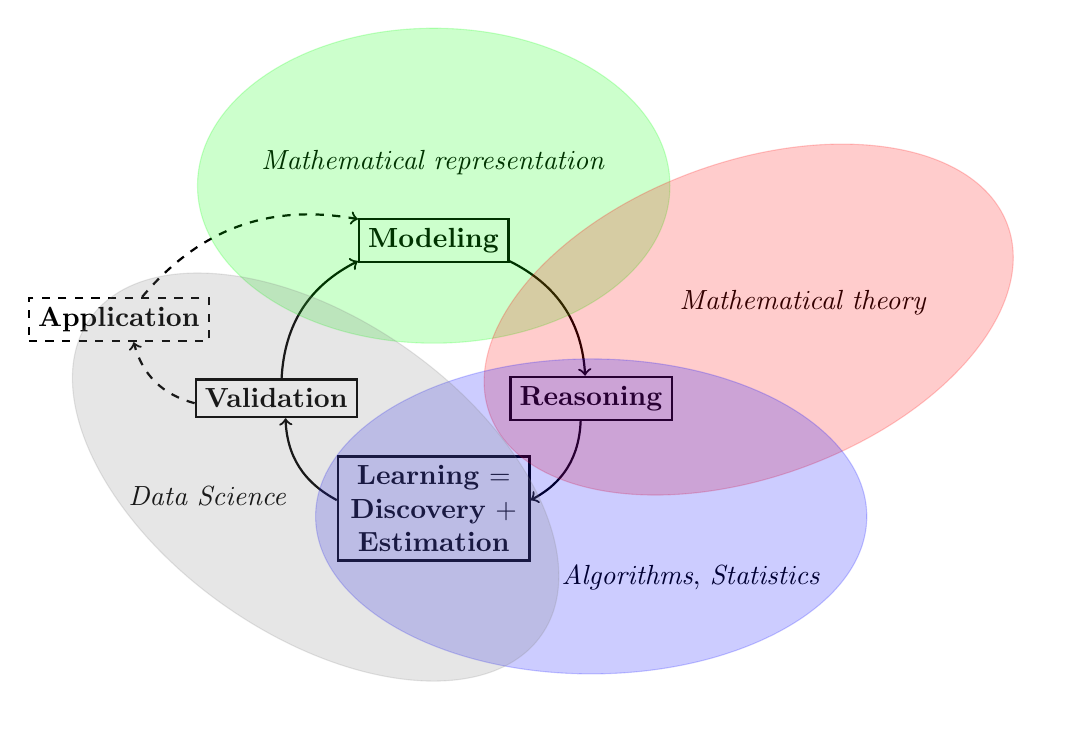
\begin{tikzpicture}
    \node[rectangle,draw,thick] (M) at (0,2) {\textbf{Modeling}};
    \node[rectangle,draw,thick] (R) at (2,0) {\textbf{Reasoning}};
    \node[rectangle,draw,thick,text width=2.2cm,text centered] (D) at (0,-1.4) {\textbf{Learning} $=$\\ \textbf{Discovery} $+$\\ \textbf{Estimation}};
    \node[rectangle,draw,thick] (V) at (-2,0) {\textbf{Validation}};
    \node[rectangle,draw,thick,dashed] (A) at (-4,1) {\textbf{Application}};
    \draw[bend left,->,thick] (M) edge (R);
    \draw[bend left,->,thick] (R) edge (D);
    \draw[bend left,->,thick] (D) edge (V);
    \draw[bend left,->,thick] (V) edge (M);
    \draw[bend left,->,thick,dashed] (V) edge (A);
    \draw[bend left,->,thick,dashed] (A) edge (M);
    %\uncover<2->{
    \node (A1) at (0,3) {\emph{Mathematical representation}};
    \node[anchor=north west] (A2) at (3,1.5) {\emph{Mathematical theory}};
    \node[anchor=north west] (A3) at (1.5,-2) {\emph{Algorithms}, \emph{Statistics}};
    \node[anchor=north west] (A4) at (-4,-1) {\emph{Data Science}};
    \draw[draw=green,fill=green,opacity=0.2] (0,2.7) ellipse (3cm and 2cm);
    \draw[draw=red,fill=red,opacity=0.2,rotate around={20:(4,1)}] (4,1) ellipse (3.5cm and 2cm);
    \draw[draw=blue,fill=blue,opacity=0.2,rotate around={0:(2,-1.5)}] (2,-1.5) ellipse (3.5cm and 2cm);
    \draw[draw=gray,fill=gray,opacity=0.2,rotate around={-35:(-1.5,-1)}] (-1.5,-1) ellipse (3.5cm and 2cm);
%    \uncover<3->{
%      \node[draw=black,fill=white,opacity=0.9,rectangle,text width=8cm,inner sep=5mm] at (1,0.1) {\textbf{Some of the challenges to be addressed:}\\ \begin{itemize}
%    \item Causal cycles (feedback loops)
%    \item Confounders (latent common causes)
%    \item Combining different datasets / contexts
%    \item Reliability vs.\ computational complexity
%    \item Selection Bias
%      \end{itemize}};}
%  }
  \end{tikzpicture}
\end{frame}

\frame{\frametitle{Example: Causal Discovery}
  \begin{example}
  Causal Discovery = Estimating the Causal Graph from Data
  \end{example}
}

\frame{\frametitle{Causal relations}
  \begin{definition}[Informal]
    Let $X$ and $Y$ be two distinct variables of system.
    \alert{$X$ causes $Y$} if changing $X$ (\emph{intervening on $X$}) leads to a change of $Y$.
  \end{definition}

  \medskip
%  \pause
  \alert{Causal graph} represents causal relationships between variables graphically.

\begin{example}
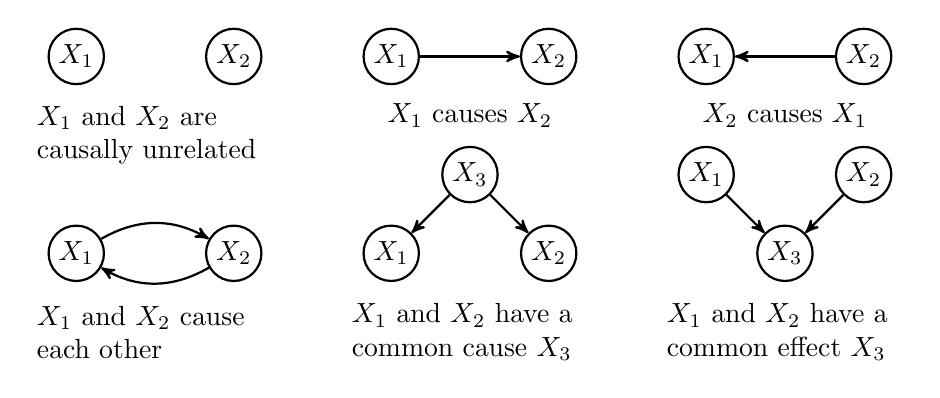
\begin{tikzpicture}
  \begin{scope}
    \node[var] (X1) at (-1,0) {$X_1$};
    \node[var] (X2) at (1,0) {$X_2$};
    \node[text width=3cm] at (0,-1.0) {$X_1$ and $X_2$ are causally unrelated};
  \end{scope}
  \begin{scope}[xshift=4cm]
    \node[var] (X1) at (-1,0) {$X_1$};
    \node[var] (X2) at (1,0) {$X_2$};
    \draw[arr] (X1) edge (X2);
    \node at (0,-0.75) {$X_1$ causes $X_2$};
  \end{scope}
  \begin{scope}[xshift=8cm]
    \node[var] (X1) at (-1,0) {$X_1$};
    \node[var] (X2) at (1,0) {$X_2$};
    \draw[arr] (X2) edge (X1);
    \node at (0,-0.75) {$X_2$ causes $X_1$};
  \end{scope}
  \begin{scope}[yshift=-2.5cm]
    \node[var] (X1) at (-1,0) {$X_1$};
    \node[var] (X2) at (1,0) {$X_2$};
    \draw[arr,bend left] (X1) edge (X2);
    \draw[arr,bend left] (X2) edge (X1);
    \node[text width=3cm] at (0,-1) {$X_1$ and $X_2$ cause each other};
  \end{scope}
  \begin{scope}[yshift=-2.5cm,xshift=4cm]
    \node[var] (X1) at (-1,0) {$X_1$};
    \node[var] (X2) at (1,0) {$X_2$};
    \node[var] (X3) at (0,1) {$X_3$};
    \draw[arr] (X3) edge (X1);
    \draw[arr] (X3) edge (X2);
    \node[text width=3cm] at (0,-1) {$X_1$ and $X_2$ have a common cause $X_3$};
  \end{scope}
  \begin{scope}[yshift=-2.5cm,xshift=8cm]
    \node[var] (X1) at (-1,1) {$X_1$};
    \node[var] (X2) at (1,1) {$X_2$};
    \node[var] (X3) at (0,0) {$X_3$};
    \draw[arr] (X1) edge (X3);
    \draw[arr] (X2) edge (X3);
    \node[text width=3cm] at (0,-1) {$X_1$ and $X_2$ have a common effect $X_3$};
  \end{scope}
\end{tikzpicture}
\end{example}
}

\frame{\frametitle{Direct causation}
Let $\B{V} = \{X_1,\dots,X_N\}$ be a set of variables.
\begin{definition}[Informal]
If $X_i$ causes $X_j$ even if all other variables $\B{V} \setminus \{X_i,X_j\}$ are hold fixed at some values, then
\begin{itemize}
\item we say that \alert{$X_i$ causes $X_j$ directly with respect to $\B{V}$}
\item we indicate this in the causal graph on $\B{V}$ by a \alert{directed edge $X_i \to X_j$}
\end{itemize}
\end{definition}

\begin{example}\small
\centering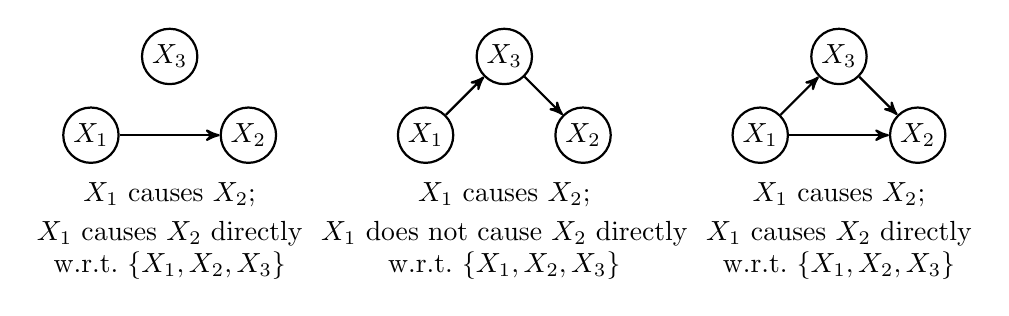
\begin{tikzpicture}
  \begin{scope}[xshift=0cm]
    \node[var] (X1) at (-1,0) {$X_1$};
    \node[var] (X2) at (1,0) {$X_2$};
    \node[var] (X3) at (0,1) {$X_3$};
    \draw[arr] (X1) edge (X2);
    \node at (0,-0.75) {$X_1$ causes $X_2$;};
    \node at (0,-1.25) {$X_1$ causes $X_2$ directly};
    \node at (0,-1.65) {w.r.t.\ $\{X_1,X_2,X_3\}$};
  \end{scope}
  \begin{scope}[xshift=4.25cm]
    \node[var] (X1) at (-1,0) {$X_1$};
    \node[var] (X2) at (1,0) {$X_2$};
    \node[var] (X3) at (0,1) {$X_3$};
    \draw[arr] (X1) edge (X3);
    \draw[arr] (X3) edge (X2);
    \node at (0,-0.75) {$X_1$ causes $X_2$;};
    \node at (0,-1.25) {$X_1$ does not cause $X_2$ directly};
    \node at (0,-1.65) {w.r.t.\ $\{X_1,X_2,X_3\}$};
  \end{scope}
  \begin{scope}[xshift=8.5cm]
    \node[var] (X1) at (-1,0) {$X_1$};
    \node[var] (X2) at (1,0) {$X_2$};
    \node[var] (X3) at (0,1) {$X_3$};
    \draw[arr] (X1) edge (X3);
    \draw[arr] (X3) edge (X2);
    \draw[arr] (X1) edge (X2);
    \node at (0,-0.75) {$X_1$ causes $X_2$;};
    \node at (0,-1.25) {$X_1$ causes $X_2$ directly};
    \node at (0,-1.65) {w.r.t.\ $\{X_1,X_2,X_3\}$};
  \end{scope}
\end{tikzpicture}
\end{example}
}

\frame{\frametitle{Direct vs.\ indirect causation: Example}
  \centerline{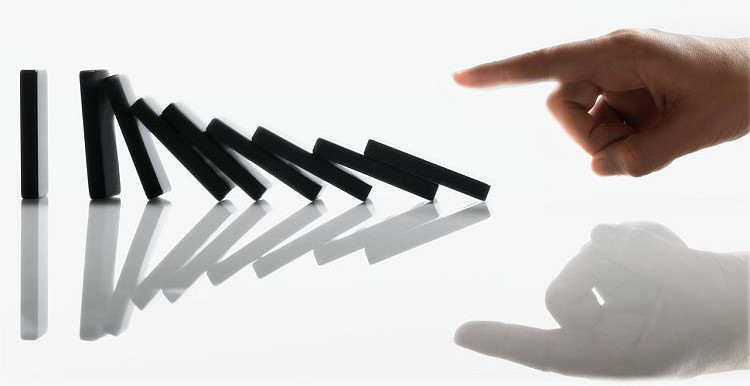
\includegraphics[width=0.8\textwidth]{domino.jpg}}
  \begin{itemize}
    \item Each stone causes \emph{all} subsequent stones to topple.
    \item Each stone only \alert{directly causes} the \alert{next} neighboring stone to topple.
    \item Causal graph:\\[0.5\baselineskip]
      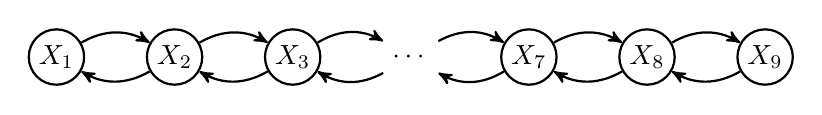
\begin{tikzpicture}
        \node[var] (X1) at (1,0) {$X_1$};
        \node[var] (X2) at (2.5,0) {$X_2$};
        \node[var] (X3) at (4,0) {$X_3$};
        \node      (dots) at (5.5,0) {$\cdots$};
        \node[var] (X7) at (7,0) {$X_7$};
        \node[var] (X8) at (8.5,0) {$X_8$};
        \node[var] (X9) at (10,0) {$X_9$};
        \draw[arr,bend left] (X2) edge (X1);
        \draw[arr,bend left] (X3) edge (X2);
        \draw[arr,bend left] (dots) edge (X3);
        \draw[arr,bend left] (X7) edge (dots);
        \draw[arr,bend left] (X8) edge (X7);
        \draw[arr,bend left] (X9) edge (X8);
        \draw[arr,bend left] (X1) edge (X2);
        \draw[arr,bend left] (X2) edge (X3);
        \draw[arr,bend left] (X3) edge (dots);
        \draw[arr,bend left] (dots) edge (X7);
        \draw[arr,bend left] (X7) edge (X8);
        \draw[arr,bend left] (X8) edge (X9);
      \end{tikzpicture}
  \end{itemize}
}

\begin{frame}{Constraint-based Causal Discovery}
  From the pattern of conditional independences in the data we can reconstruct
  a set of possible underlying causal graphs, \emph{even when allowing for latent confounders} (Spirtes, Gleimour, Scheines; 2000).

  \bigskip
\centerline{\scalebox{1.0}{\begin{tikzpicture}
  \node[label=Data,rectangle,draw=blue] (AA) at (-1,0) {\scalebox{0.7}{\begin{tabular}[t]{|cccc|}
\hline
$X_1$ & $X_2$ & $X_3$ & $X_4$ \\
\hline
  2 & 0.1  & 0.2 & 0.5\\
  2 & 0.13 & 0.21 & 0.49\\
  2 & 0.23 & 0.21 & 0.51\\
  5 & 0.5 & 0.19 & 0.52\\
  5 & 0.6 & 0.18 & 0.51\\
  2 & 0.2 & 0.22 & 0.92\\
  2 & 0.23 & 0.21 & 0.99\\
  5 & 0.53 & 1.2 & 0.95\\
%  5 & 0.61 & 1.21 & 0.90\\
  5 & 0.55 & 1.19 & 0.97\\
\hline
    \end{tabular}}};
    \node[label=CIs,rectangle,draw=blue,text width=1.8cm] (BB) at (3,0) {\small $X_2 \notindep X_4$\\ $X_2 \indep X_4 \given X_3$\\ $X_1 \indep X_2$ \\ $X_1 \notindep X_2 \given X_3$\\ $\dots$};
    \draw[->, >=latex, line width=3pt] (AA) edge (BB);
    \node[rectangle,draw=blue,label=Possible Causal Graphs] (DD) at (7,0) {\scalebox{0.5}{\begin{tikzpicture}
      \begin{scope}
        \node[var] (X1) at (-1,0) {$X_1$};
        \node[var] (X2) at (1,0)  {$X_2$};
        \node[var] (X3) at (0,-1) {$X_3$}; 
        \node[var] (X4) at (0,-2.5) {$X_4$}; 
        \draw[arr] (X1) edge (X3);
        \draw[arr] (X2) edge (X3);
        \draw[arr] (X3) edge (X4);
      \end{scope}
      \begin{scope}[xshift=3.5cm]
        \node[var] (X1) at (-1,0) {$X_1$};
        \node[var] (X2) at (1,0)  {$X_2$};
        \node[var] (X3) at (0,-1) {$X_3$}; 
        \node[var] (X4) at (0,-2.5) {$X_4$}; 
        \draw[biarr] (X1) edge (X3);
        \draw[arr] (X2) edge (X3);
        \draw[arr] (X3) edge (X4);
      \end{scope}
      \begin{scope}[yshift=-4cm]
        \node[var] (X1) at (-1,0) {$X_1$};
        \node[var] (X2) at (1,0)  {$X_2$};
        \node[var] (X3) at (0,-1) {$X_3$}; 
        \node[var] (X4) at (0,-2.5) {$X_4$}; 
        \draw[biarr,bend left] (X1) edge (X3);
        \draw[arr] (X1) edge (X3);
        \draw[arr] (X2) edge (X3);
        \draw[arr] (X3) edge (X4);
      \end{scope}
      \begin{scope}[xshift=3.5cm,yshift=-4cm]
%        \node at (0,-1.5) {$\dots$};
        \node at (0,-1.5) {\scalebox{0.4}{\begin{tikzpicture}
          \begin{scope}
            \node[var] (X1) at (-1,0) {$X_1$};
            \node[var] (X2) at (1,0)  {$X_2$};
            \node[var] (X3) at (0,-1) {$X_3$}; 
            \node[var] (X4) at (0,-2.5) {$X_4$}; 
            \draw[arr] (X1) edge (X3);
            \draw[biarr] (X2) edge (X3);
            \draw[arr] (X3) edge (X4);
          \end{scope}
          \begin{scope}[xshift=3.5cm]
            \node[var] (X1) at (-1,0) {$X_1$};
            \node[var] (X2) at (1,0)  {$X_2$};
            \node[var] (X3) at (0,-1) {$X_3$}; 
            \node[var] (X4) at (0,-2.5) {$X_4$}; 
            \draw[biarr] (X1) edge (X3);
            \draw[biarr] (X2) edge (X3);
            \draw[arr] (X3) edge (X4);
          \end{scope}
          \begin{scope}[yshift=-4cm]
            \node[var] (X1) at (-1,0) {$X_1$};
            \node[var] (X2) at (1,0)  {$X_2$};
            \node[var] (X3) at (0,-1) {$X_3$}; 
            \node[var] (X4) at (0,-2.5) {$X_4$}; 
            \draw[biarr,bend left] (X1) edge (X3);
            \draw[arr] (X1) edge (X3);
            \draw[biarr] (X2) edge (X3);
            \draw[arr] (X3) edge (X4);
          \end{scope}
          \begin{scope}[xshift=3.5cm,yshift=-4cm]
            \node at (0,-1.5) {\scalebox{0.4}{\begin{tikzpicture}
              \begin{scope}
                \node[var] (X1) at (-1,0) {$X_1$};
                \node[var] (X2) at (1,0)  {$X_2$};
                \node[var] (X3) at (0,-1) {$X_3$}; 
                \node[var] (X4) at (0,-2.5) {$X_4$}; 
                \draw[arr] (X1) edge (X3);
                \draw[biarr,bend left] (X2) edge (X3);
                \draw[arr] (X2) edge (X3);
                \draw[arr] (X3) edge (X4);
              \end{scope}
              \begin{scope}[xshift=3.5cm]
                \node[var] (X1) at (-1,0) {$X_1$};
                \node[var] (X2) at (1,0)  {$X_2$};
                \node[var] (X3) at (0,-1) {$X_3$}; 
                \node[var] (X4) at (0,-2.5) {$X_4$}; 
                \draw[biarr] (X1) edge (X3);
                \draw[biarr,bend left] (X2) edge (X3);
                \draw[arr] (X2) edge (X3);
                \draw[arr] (X3) edge (X4);
              \end{scope}
              \begin{scope}[yshift=-4cm]
                \node[var] (X1) at (-1,0) {$X_1$};
                \node[var] (X2) at (1,0)  {$X_2$};
                \node[var] (X3) at (0,-1) {$X_3$}; 
                \node[var] (X4) at (0,-2.5) {$X_4$}; 
                \draw[biarr,bend left] (X1) edge (X3);
                \draw[arr] (X1) edge (X3);
                \draw[biarr,bend left] (X2) edge (X3);
                \draw[arr] (X2) edge (X3);
                \draw[arr] (X3) edge (X4);
              \end{scope}
            \end{tikzpicture}}};
          \end{scope}
        \end{tikzpicture}}};
      \end{scope}
    \end{tikzpicture}}};
    \draw[->, >=latex, line width=3pt] (BB) -- (DD);
  \end{tikzpicture}}
  }

  Modern algorithms can deal with: latent confounding, selection bias, causal cycles, combining various data sources.
%\pause
%\bigskip
%\cite{ForreMooij_UAI_18}: the first causal discovery algorithm that can handle
%cycles, nonlinear relationships, latent (confounding) variables and data from different (interventional) contexts.
\end{frame}


\frame[t]{\frametitle{Problem 1: Understanding Protein Signaling}
%\begin{example}
%\centering  How to infer a signaling network from single-cell data?
%  \bigskip
  \centering\begin{tikzpicture}
    \draw[rounded corners] (-3.1,-4.7) rectangle (3.1,3.3);
    \draw[rounded corners] (5,-4.7) rectangle (9,3.3);
    \node at (0,3)    {\large Protein Abundance Data:};
    \node at (0,2.5)  {\footnotesize (Sachs \emph{et al}, 2005)};
    \node at (0,0.1)  {\includegraphics[height=4cm]{sachs_data}};
    \node at (0,-3.4) {\tiny \begin{tabular}{cll}
                        Condition & Reagent & Intervention \\
                        \hline
                        1 & - & observational \\
                        2 & Akt-inhibitor & inhibits AKT activity \\
                        3 & G0076 & inhibits PKC activity \\
                        4 & Psitectorigenin & inhibits PIP2 abundance \\
                        5 & U0126 & inhibits MEK activity \\
                        6 & LY294002 & inhibits PIP2/PIP3 activity \\
                        7 & PMA & activates PKC + global \\
                        8 & $\beta$2CAMP & activates PKA + global
                      \end{tabular}};
    \node at (7,3)   {\large Causal Graph:};
    \node at (7,2.5) {\footnotesize (``Signalling network'')};
    \node at (7,-1)  {\includegraphics[width=3.7cm]{sachs_gt}};
    \node at (7,-4.5) {\tiny (depicted here: ``consensus'' network)};
    \draw[->, >=latex, line width=6pt] (3.3,-0.8) -- (4.8,-0.8);
%    \node at (4.0,0) {\huge ?};
  \end{tikzpicture}
%\end{example}
}

\begin{frame}{Causal Discovery Results}
  \begin{tikzpicture}
%    \node at (0,-0.25) {\includegraphics[width=0.4\textwidth]{sachs-fci-obs-pag.pdf}};
%    \node at (0,1.5) {Only observational data (FCI):};
    \node at (4,-4) {\includegraphics[width=0.7\textwidth]{sachs-fci-jci123-pag.pdf}};
%    \node at (4,-1.75) {All data (FCI-JCI), learned intervention targets:};
%    \node at (0,-6) {\includegraphics[width=0.5\textwidth]{sachs-gt.pdf}};
%    \node at (0,-4.75) {``Consensus'' (Sachs \emph{et al.}, 2005)};
  \end{tikzpicture}

  \bigskip
  But what is the ``true'' causal structure?
\end{frame}

\begin{frame}{Gene Regulatory Network = Causal Graph}\centering
  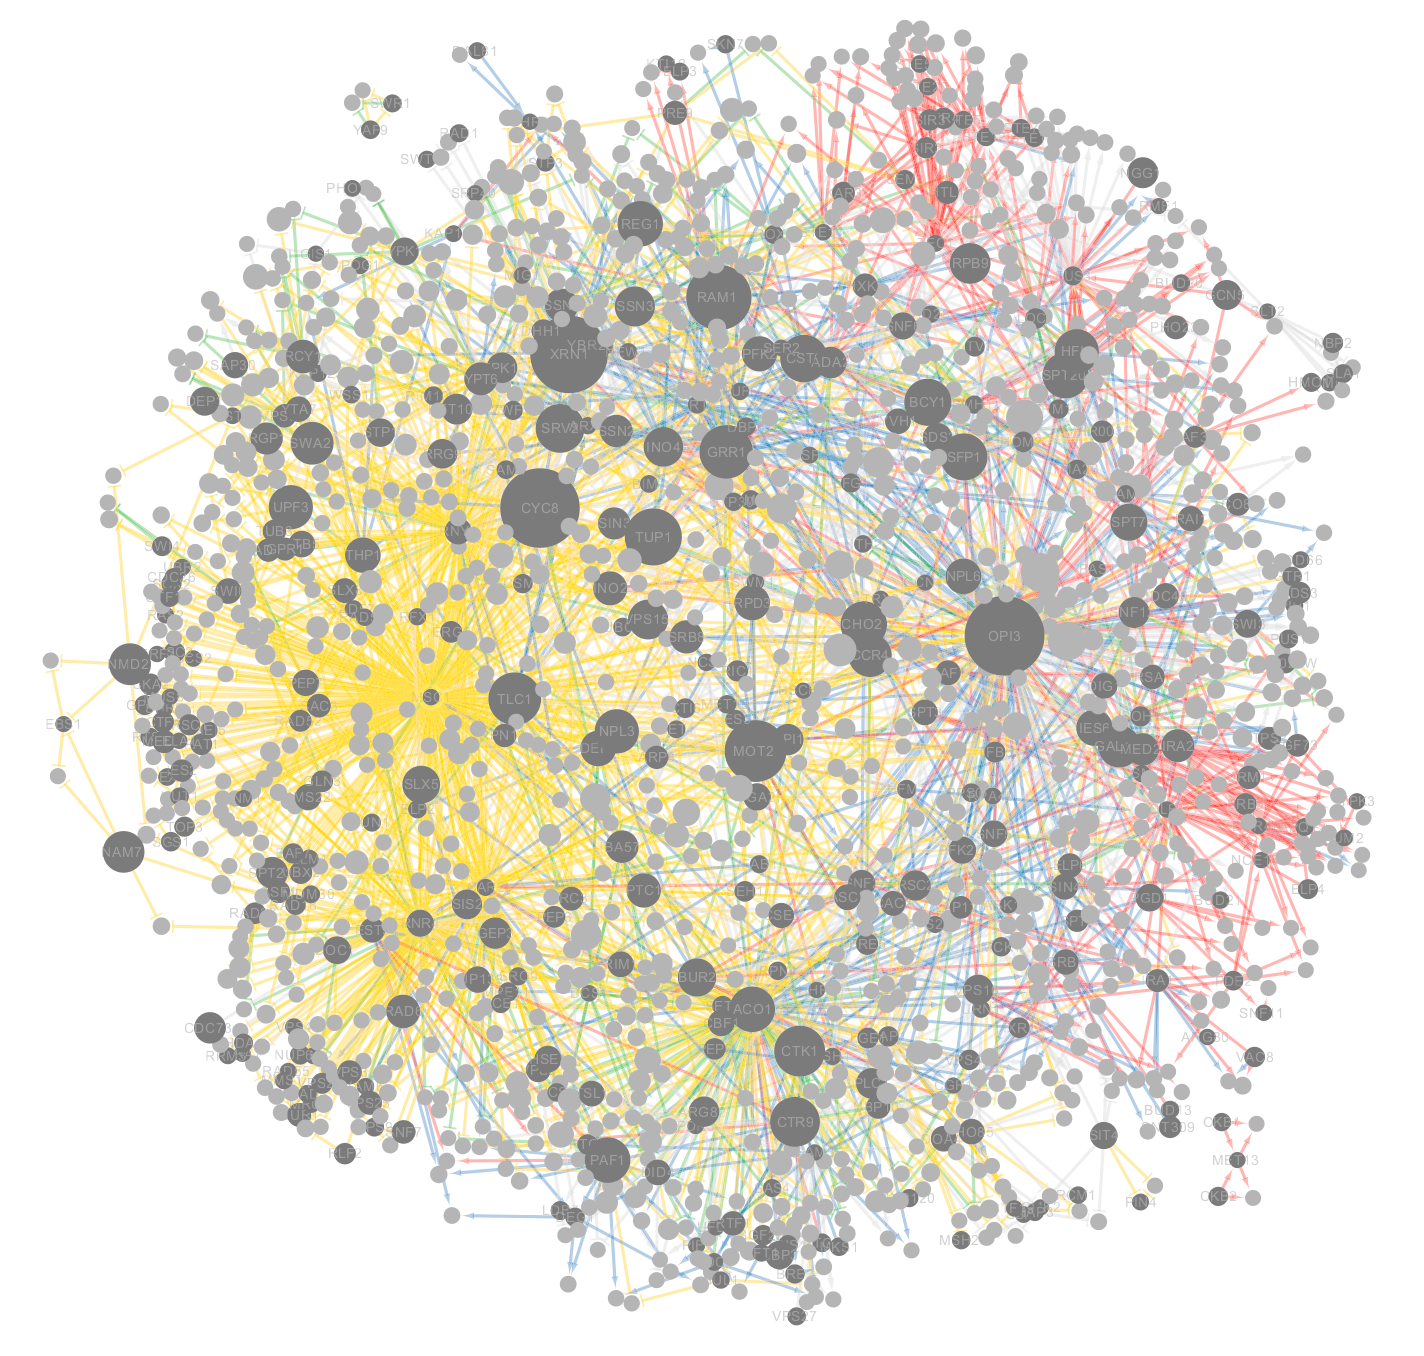
\includegraphics[width=0.7\textwidth]{yeast_gene_regulatory_network_Kemmeren.png}
  %\vspace{-5cm}
  {\tiny Source: Kemmeren \emph{et al}, 2014}
\end{frame}

%\setbeamertemplate{background}{\includegraphics[width=\paperwidth,height=\paperheight,keepaspectratio]{yeast}}
\begin{frame}{Problem 2: Causal Discovery of Gene Regulatory Networks}
  \begin{topalignedcolumn}{0.35\textwidth}
  \vspace{-5mm}
  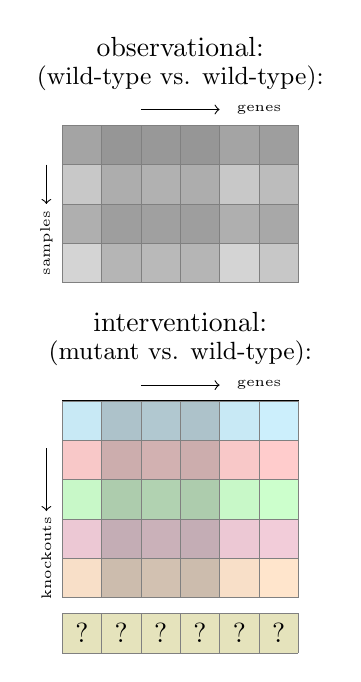
\begin{tikzpicture}
    \begin{scope}
      \node at (1.5,3) {observational:};
      \node at (1.5,2.6) {\small (wild-type vs. wild-type):};
      \draw[draw=none,fill=gray!30!white] (0,0.0) rectangle (3,0.5);
      \draw[draw=none,fill=gray!60!white] (0,0.5) rectangle (3,1.0);
      \draw[draw=none,fill=gray!40!white] (0,1.0) rectangle (3,1.5);
      \draw[draw=none,fill=gray!70!white] (0,1.5) rectangle (3,2.0);
      \draw[draw=none,opacity=0.05,fill=gray] (0.0,0) rectangle (0.5,2);
      \draw[draw=none,opacity=0.40,fill=gray] (0.5,0) rectangle (1.0,2);
      \draw[draw=none,opacity=0.35,fill=gray] (1.0,0) rectangle (1.5,2);
      \draw[draw=none,opacity=0.40,fill=gray] (1.5,0) rectangle (2.0,2);
      \draw[draw=none,opacity=0.05,fill=gray] (2.0,0) rectangle (2.5,2);
      \draw[draw=none,opacity=0.20,fill=gray] (2.5,0) rectangle (3.0,2);
      \draw (0,0) rectangle (3,2);
      \draw[step=5mm,gray,very thin] (0,0) grid (3,2);
      \draw[->] (1,2.2) -- (2,2.2);
      \node at (2.5,2.2) {\tiny genes};
      \draw[->] (-0.2,1.5) -- (-0.2,1.0);
      \node[rotate=90] at (-0.2,0.5) {\tiny samples};
    \end{scope}
    \begin{scope}[yshift=-4.5cm]
      \node at (1.5,4) {interventional:};
      \node at (1.5,3.6) {\small (mutant vs. wild-type):};
      \draw[draw=none,fill=orange!20!white] (0,0.5) rectangle (3,1.0);
      \draw[draw=none,fill=purple!20!white] (0,1.0) rectangle (3,1.5);
      \draw[draw=none,fill=green!20!white] (0,1.5) rectangle (3,2.0);
      \draw[draw=none,fill=red!20!white] (0,2.0) rectangle (3,2.5);
      \draw[draw=none,fill=cyan!20!white] (0,2.5) rectangle (3,3.0);
%      \draw[draw=none,fill=gray!10!white] (0,0.0) rectangle (3,0.5);
%      \draw[draw=none,fill=gray!30!white] (0,0.5) rectangle (3,1.0);
%      \draw[draw=none,fill=gray!20!white] (0,1.0) rectangle (3,1.5);
%      \draw[draw=none,fill=gray!50!white] (0,1.5) rectangle (3,2.0);
%      \draw[draw=none,fill=gray!10!white] (0,2.0) rectangle (3,2.5);
%      \draw[draw=none,fill=gray!20!white] (0,2.5) rectangle (3,3.0);
      \draw[draw=none,opacity=0.05,fill=gray] (0.0,0.5) rectangle (0.5,3);
      \draw[draw=none,opacity=0.40,fill=gray] (0.5,0.5) rectangle (1.0,3);
      \draw[draw=none,opacity=0.35,fill=gray] (1.0,0.5) rectangle (1.5,3);
      \draw[draw=none,opacity=0.40,fill=gray] (1.5,0.5) rectangle (2.0,3);
      \draw[draw=none,opacity=0.05,fill=gray] (2.0,0.5) rectangle (2.5,3);
%      \draw[draw=none,opacity=0.20,fill=gray] (2.5,0.5) rectangle (3.0,3);
      \draw (0,0.5) rectangle (3,3);
      \draw[step=5mm,gray,very thin] (0,0.5) grid (3,3);
      \draw[->] (1,3.2) -- (2,3.2);
      \node at (2.5,3.2) {\tiny genes};
      \draw[->] (-0.2,2.4) -- (-0.2,1.6);
      \node[rotate=90] at (-0.2,1) {\tiny knockouts};
      \uncover<2-2>{\begin{scope}[yshift=-0.2cm]
      \draw (0,0.0) rectangle (3,0.5);
      \draw[draw=none,fill=yellow!20!white] (0,0.0) rectangle (3,0.5);
      \draw[step=5mm,gray,very thin] (0,0.0) grid (3,0.5);
      \draw[draw=none,opacity=0.20,fill=gray] (0.0,0.0) rectangle (3.0,0.5);
      \node at (0.25,0.25) {?};
      \node at (0.75,0.25) {?};
      \node at (1.25,0.25) {?};
      \node at (1.75,0.25) {?};
      \node at (2.25,0.25) {?};
      \node at (2.75,0.25) {?};
      \end{scope}}
    \end{scope}
    \begin{scope}
    \end{scope}
  \end{tikzpicture}
  \end{topalignedcolumn}\ %
  \begin{topalignedcolumn}{0.62\textwidth}
    Large-scale Single Gene Knockout Micro-Array Data:
    \begin{itemize}
      \item $\sim$6,500 variables (gene expression)
      \item $\sim$260 observational samples (wild-type vs.\ wild-type)
      \item $\sim$1,500 interventional samples (single-gene knockouts/knockdowns)
    \end{itemize}

%    \bigskip
%    ``Reconstructing gene regulatory network'' ${}={}$ causal discovery

    \uncover<2-2>{\begin{block}{Challenge}Can we, in a purely data-driven way (without using biological knowledge), predict which genes strongly change their expression when we knock-out a given gene (without using any data corresponding to that particular knock-out experiment)?
    \end{block}}

%    \begin{itemize}
%      \item Predict from observational data, validate using interventional data
%      \item Predict from combination of observational and interventional data,
%        validate using hold-out interventional data
%    \end{itemize}
  \end{topalignedcolumn}
\end{frame}

\begin{frame}{Causation or correlation?}
  \begin{tikzpicture}
  \node at (0,0) {Causal:};
  \node at (6,0) {Non-causal:};
  \node at (0,-2.7) {\includegraphics[width=0.45\textwidth]{01_YPL273W_vs_YMR321C.pdf}};
    \node at (6,-2.7) {\includegraphics[width=0.45\textwidth]{38_YPL154C_vs_YDR032C.pdf}};
  \end{tikzpicture}
  \centerline{\small (Training data: {\color{blue}Observational} and {\color{red}Interventional}. Test data: {\color{green}single intervention}.)}

  \bigskip
  Causal discovery algorithms can indeed solve this!
%  \bigskip
%  Idea: introduce binary context variable ({\color{blue}$C = 0$: observational}; {\color{red}$C = 1$: interventional})
%  \cite{Meinshausen++_PNAS_16}.
  
%  \medskip
%  We can apply causal discovery methods based on simple causal background knowledge: the decision whether or not
%  to knockout a gene has been made before measuring gene expression levels.
\end{frame}

\begin{frame}{First convincing large-scale validations}
  \centerline{\includegraphics[width=0.45\textwidth]{{tpfp_xlim500_ylim30_abs_norm_prev1.00_set_joris_talk_2020_v1}.pdf}
  \includegraphics[width=0.45\textwidth]{{tpfp_xlim500_ylim30_sgd_physical_curated_prev0.06_set_joris_talk_2020_v1}.pdf}}
  \small Prediction Error (Internal Validation), \qquad SGD DB (External Validation)

%  \bigskip
%  \small {\color{blue}ICP};\\
%  {\color{green!50!black}LCD}

  \bigskip
  It works! (But can we get more predictions?)

  \bigskip
  At the end of this course, you will be able to apply LCD to this data yourself (and try to outperform the state-of-the-art!).
\end{frame}

%\frame[allowframebreaks]{\frametitle{References}
%\centerline{\huge Thank you for your attention!}
%  \begin{itemize}
%    \item J. Pearl: "Causal inference in statistics: An overview", Statistics Surveys, 3 (2009), pp. 96-146
%    \item J. Pearl: "Causality: Models, Reasoning, and Inference", Cambridge University Press, 2000
%    \item P. Spirtes, C. Glymour, R. Scheines: "Causation, Prediction, and Search", The MIT Press, 2000
%  \end{itemize}
%  \nocite{Pearl09,Pearl99,SpirtesGlymourScheines00,PJS2017}
%  \nocite{Bongers++_1611.06221v3}
%  \nocite{ForreMooij_1710.08775} 
%  \bibliographystyle{apalike}
%  \tiny
%  \bibliography{2021_uva_ias,../../bib/mooij.bib}
%}
\begin{frame}{Logistics for this course}
  \begin{itemize}
    \item Two periods
    \item No text book; lecture notes are being written and will be made available on weekly basis
    \item Lectures (Tuesdays/Mondays) via Zoom
    \item Some of the lectures will be pre-recorded and made available via Canvas
    \item Other lectures will be live (and recorded)
    \item Exercise sessions (Thursdays) via MS Teams
    \item Homework exercises will be (partially) graded
    \item Grading: 15\% exercises, 85\% exam
  \end{itemize}

  \bigskip
  Questions?
\end{frame}

\end{document}
